\documentclass{article}
\usepackage{hyperref}
\usepackage{graphicx}
\usepackage{listings}

\lstset{breaklines=true}

\begin{document}
\title{CrossCorr parameter space double-cone \\ 
LIGO-T1600313}
\author{Grant David Meadors}
\date{\today}
%\affiliation{AEI Hannover/Golm}

\maketitle

CrossCorr's 3D parameter space (frequency $f$, projected semi-major axis $a \sin i$, time of ascension $t_\mathrm{asc}$) includes a double-cone structure around simulated signals. 
On this cone, test statististc $\rho$ values are significantly higher than background, but less than the maximum. 
This structure can be considered a long-range correlation. 
While the metric approximation should not be expected to hold on the cone, the cone equation is derivable from degeneracies in the signal model. 
We illustrate this equation with figures and compare results to the corresponding $X$-pattern found in TwoSpect.

\section{Introduction}

A. Neunzert is currently investigating $X$-structures [LIGO-G1600577] in the TwoSpect pattern space that have been recently documented \hyperref[https://dx.doi.org/10.1088/0264-9381/33/10/105017]{[\textit{Classical and Quantum Gravity} \textbf{31} (2016) 105017]}.
Figure~\ref{TwoSpectGraph} illustrates such an $X$.
This structure is prominent in both the test statistic, $R$, and extrapolated single-template $\log_{10} p$-value (latter shown).
Here we note how investigations into CrossCorr [\textit{Physical Review D} \textbf{91} (2015) 102005] show that an analogous, conical feature exists for the test statistic $\rho$ in the ($f$, $a \sin i$, $t_\mathrm{asc})$ paremeter space.
While this long-range correlated structure should not be expected to be predicted by the metric approximation about peak $\rho$, it is a predictable consequence of the signal model.
Similar structures can reasonably be expected from other binary continuous-wave searches.

Scripts and plots are hosted on Atlas:

\begin{center}
\url{<
https://www.atlas.aei.uni-hannover.de/~grant.meadors/LSC/ScoX1/2016/07/21-CrossCorr/
>}
\end{center}

\noindent They are also copied in the \texttt{plots} and \texttt{scripts} directories accompanying the source for this report.
Appendix~\ref{source_code_appendix} contains the source code, with automatic linebreaks provided by the \LaTeX~\texttt{listings} package.
\noindent CrossCorr settings 
are logged in 
\texttt{log\_crosscorr.txt}. 
For example,
$T_\mathrm{sft}$ = 840 s, \texttt{maxLag} = 840 s, to aid direct comparison with TwoSpect.
The scripts are
\begin{itemize}
    \item \texttt{wrapCrossCorr.py}\\
      (wrapper function, itself called as in \texttt{example-TwoSpect-like.txt})
    \item \texttt{libCallCC.py}\\
      (functions for the wrapper)
    \item \texttt{createHeatmap.py}\\
      (grapher)
\end{itemize}

\noindent Note that we plot $\Delta f_\mathrm{obs}$,

\begin{equation} 
\Delta f_\mathrm{obs} = \frac{2 \pi a_p}{P} f,
\end{equation}

\noindent with $a_p = (a \sin i)/c$ and orbital period $P = 2 \pi / \Omega$.
This convention facilitates easier comparison.

\begin{figure}
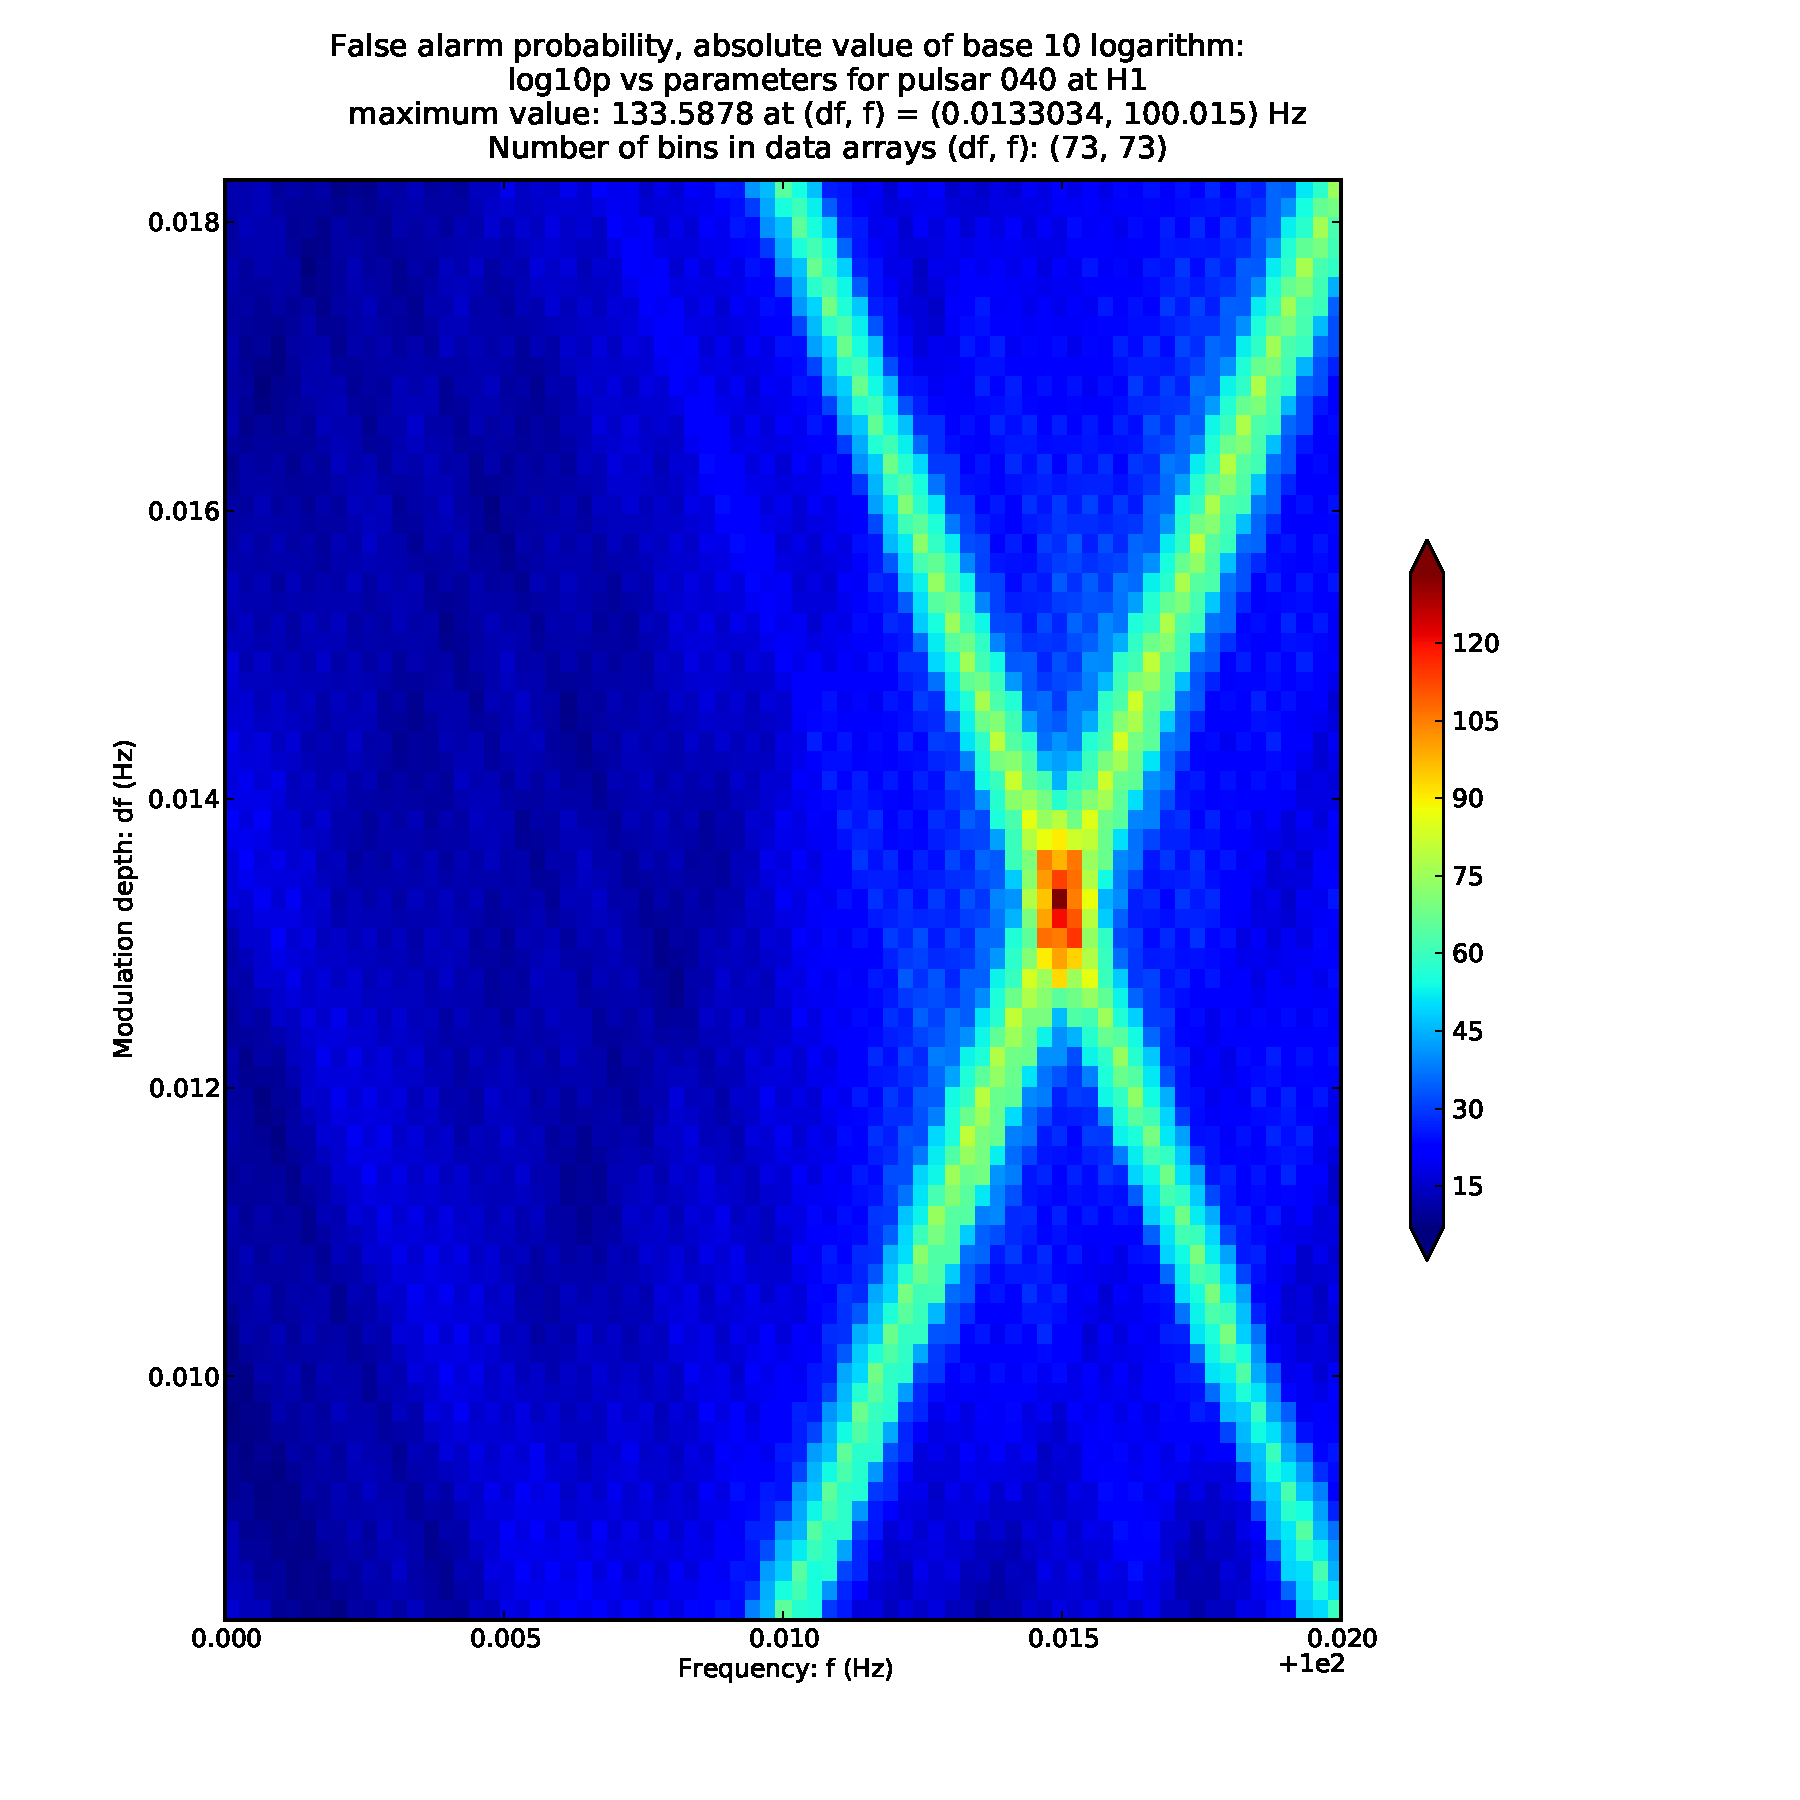
\includegraphics[trim= 0 0 0 0, clip, width=0.80\paperwidth,keepaspectratio]{plots/DFvsFresultsProb-H1_pulsar-040.pdf}
\caption{
\url{<
https://ldas-jobs.ligo-wa.caltech.edu/~gmeadors/TwoSpect/2014/06/18/injections/graph-H1-40e-26-TSni/DFvsFresultsProb-H1_pulsar-040.pdf
>}
}
\label{TwoSpectGraph}
\end{figure}

\section{Illustrations}

We take 2D slices through the 3D CrossCorr parameter space.
These dimensions are referenced by one-letter shorthand: F for $f$, A for $a_p$, T for $t_\mathrm{asc}$.
For ease of comparison, $\Delta f_\mathrm{obs} \propto a_p$ is actually graphed for A.
Each slice preserves F-A-T cyclic order, meaning that we graph the FA, AT, and TF planes along $xy$-axes.
Injection parameters are listed in Table~\ref{injection_table}; \texttt{lalapps\_Makefakedata\_v5} generated the injection.


\begin{center}
\begin{table}
\begin{tabular}{lr}
\textbf{Parameter} & \textbf{Value}\\
\hline
\texttt{Alpha} & 4.2756992385\\
\texttt{Delta} & -0.272973858335\\
\texttt{refTime} & 1245974416.0\\
\texttt{Freq} & 100.015\\
\texttt{h0} & 4e-25\\
\texttt{cosi} & 0.96724721146\\
\texttt{psi} & 5.71141493942\\
\texttt{phi0} & 4.11462142958\\
\texttt{orbitasini} & 1.44\\
\texttt{orbitEcc} & 0.0\\
\texttt{orbitTp} & 1245967532.76\\
\texttt{orbitPeriod} & 68023.82\\
\texttt{orbitArgp} & 0.0\\
\hline
\texttt{Tsft} & 840\\
\texttt{maxLag} & 840\\
\texttt{sqrtSx} & 4e-24\\
\hline
\textit{(duration)} & 1e6
\end{tabular}
\label{injection_table}
\caption{Injection parameters}
\end{table}
\end{center}



\subsection{Slices through injection center}



\begin{figure}
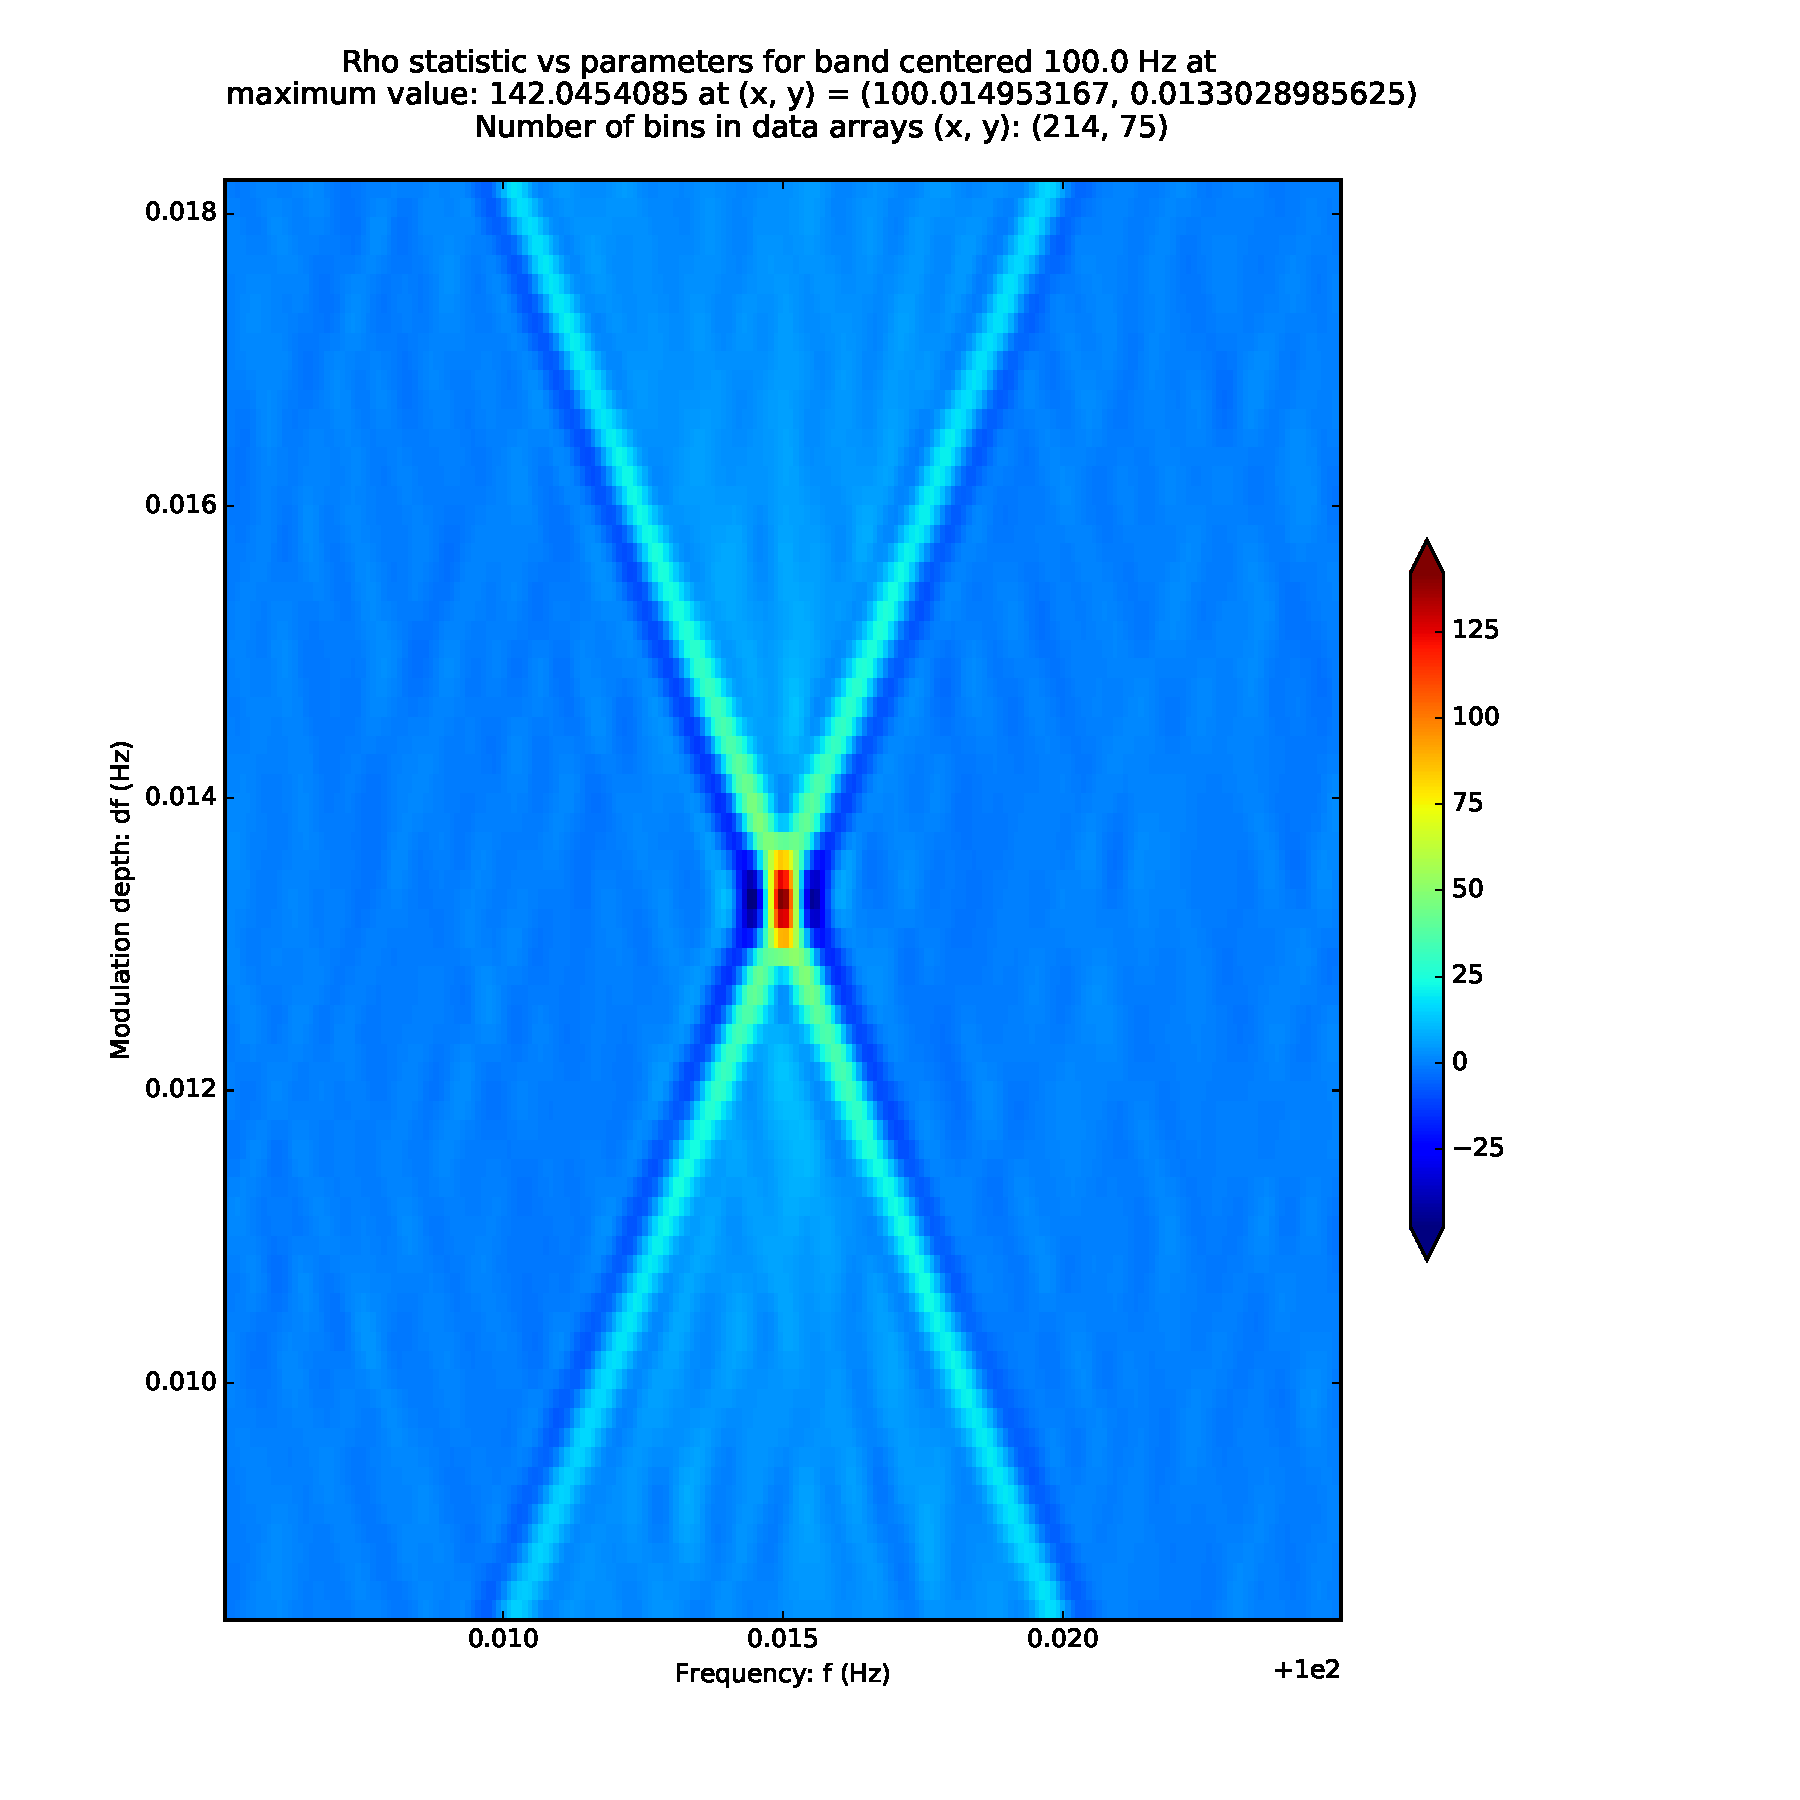
\includegraphics[trim= 0 0 0 0, clip, width=0.80\paperwidth,keepaspectratio]{plots/match-TS/FAresultsR-band-100-0.pdf}
\caption{
\url{<
https://www.atlas.aei.uni-hannover.de/~grant.meadors/LSC/ScoX1/2016/07/21-CrossCorr/match-TS/FAresultsR-band-100.0.pdf
>}
}
\label{FAcenterGraph}
\end{figure}
\begin{figure}
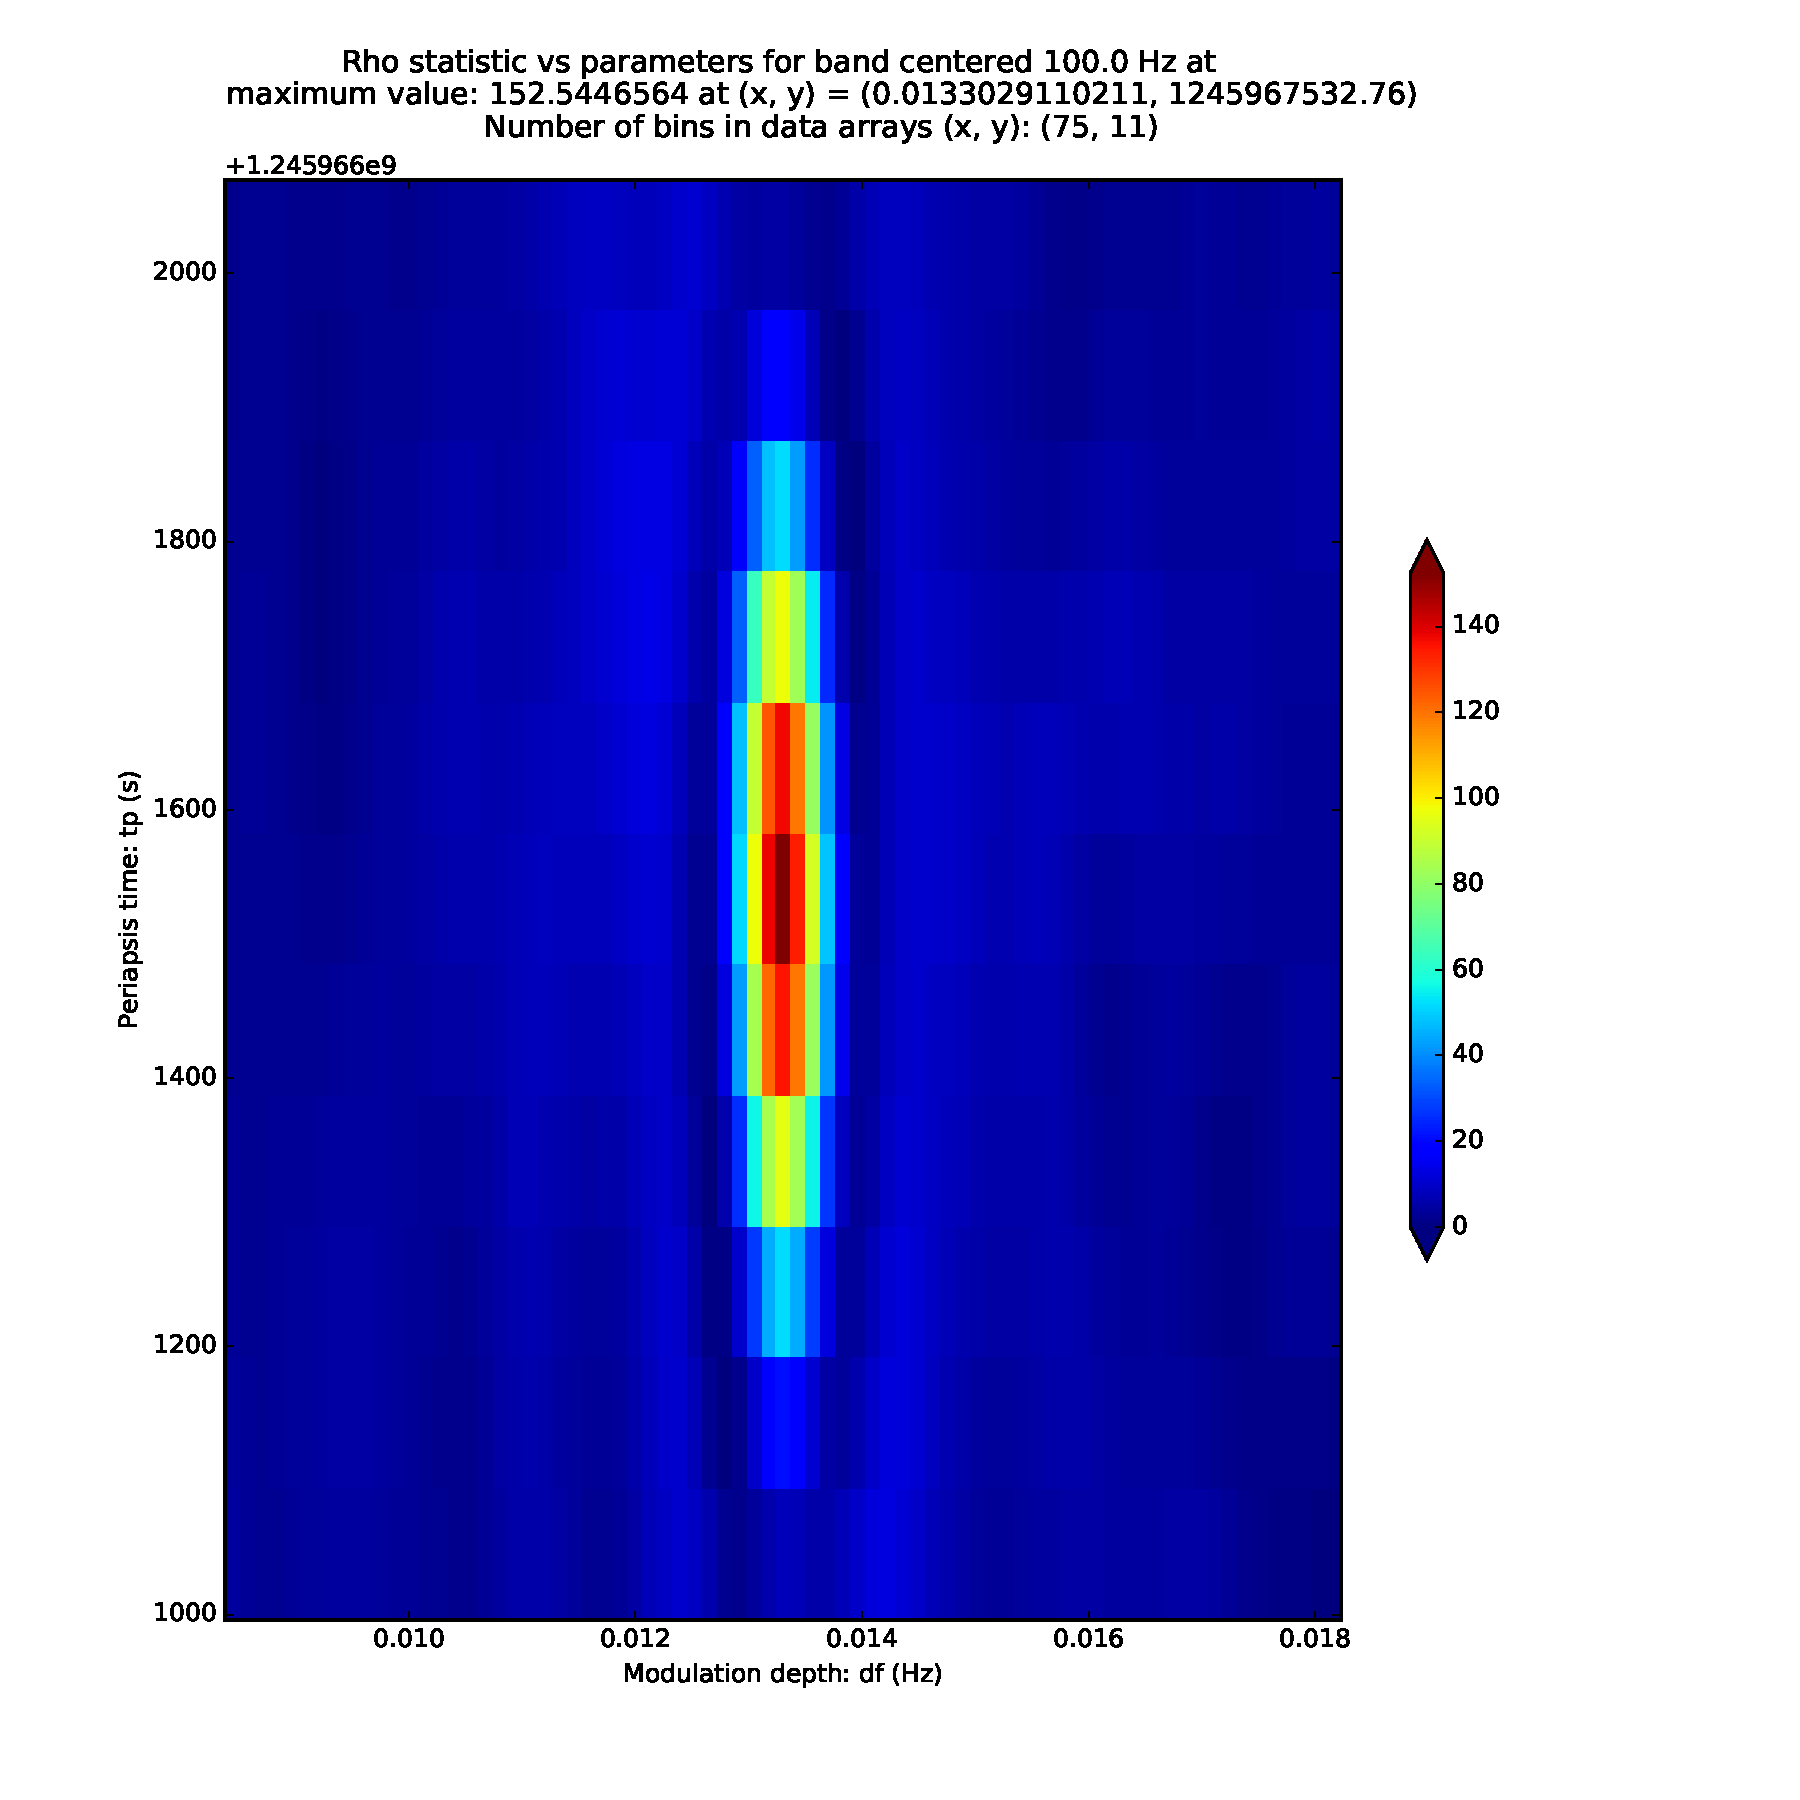
\includegraphics[trim= 0 0 0 0, clip, width=0.80\paperwidth,keepaspectratio]{plots/match-TS/ATresultsR-band-100-0.pdf}
\caption{
\url{<
https://www.atlas.aei.uni-hannover.de/~grant.meadors/LSC/ScoX1/2016/07/21-CrossCorr/match-TS/ATresultsR-band-100.0.pdf
>}
}
\label{ATcenterGraph}
\end{figure}
\begin{figure}
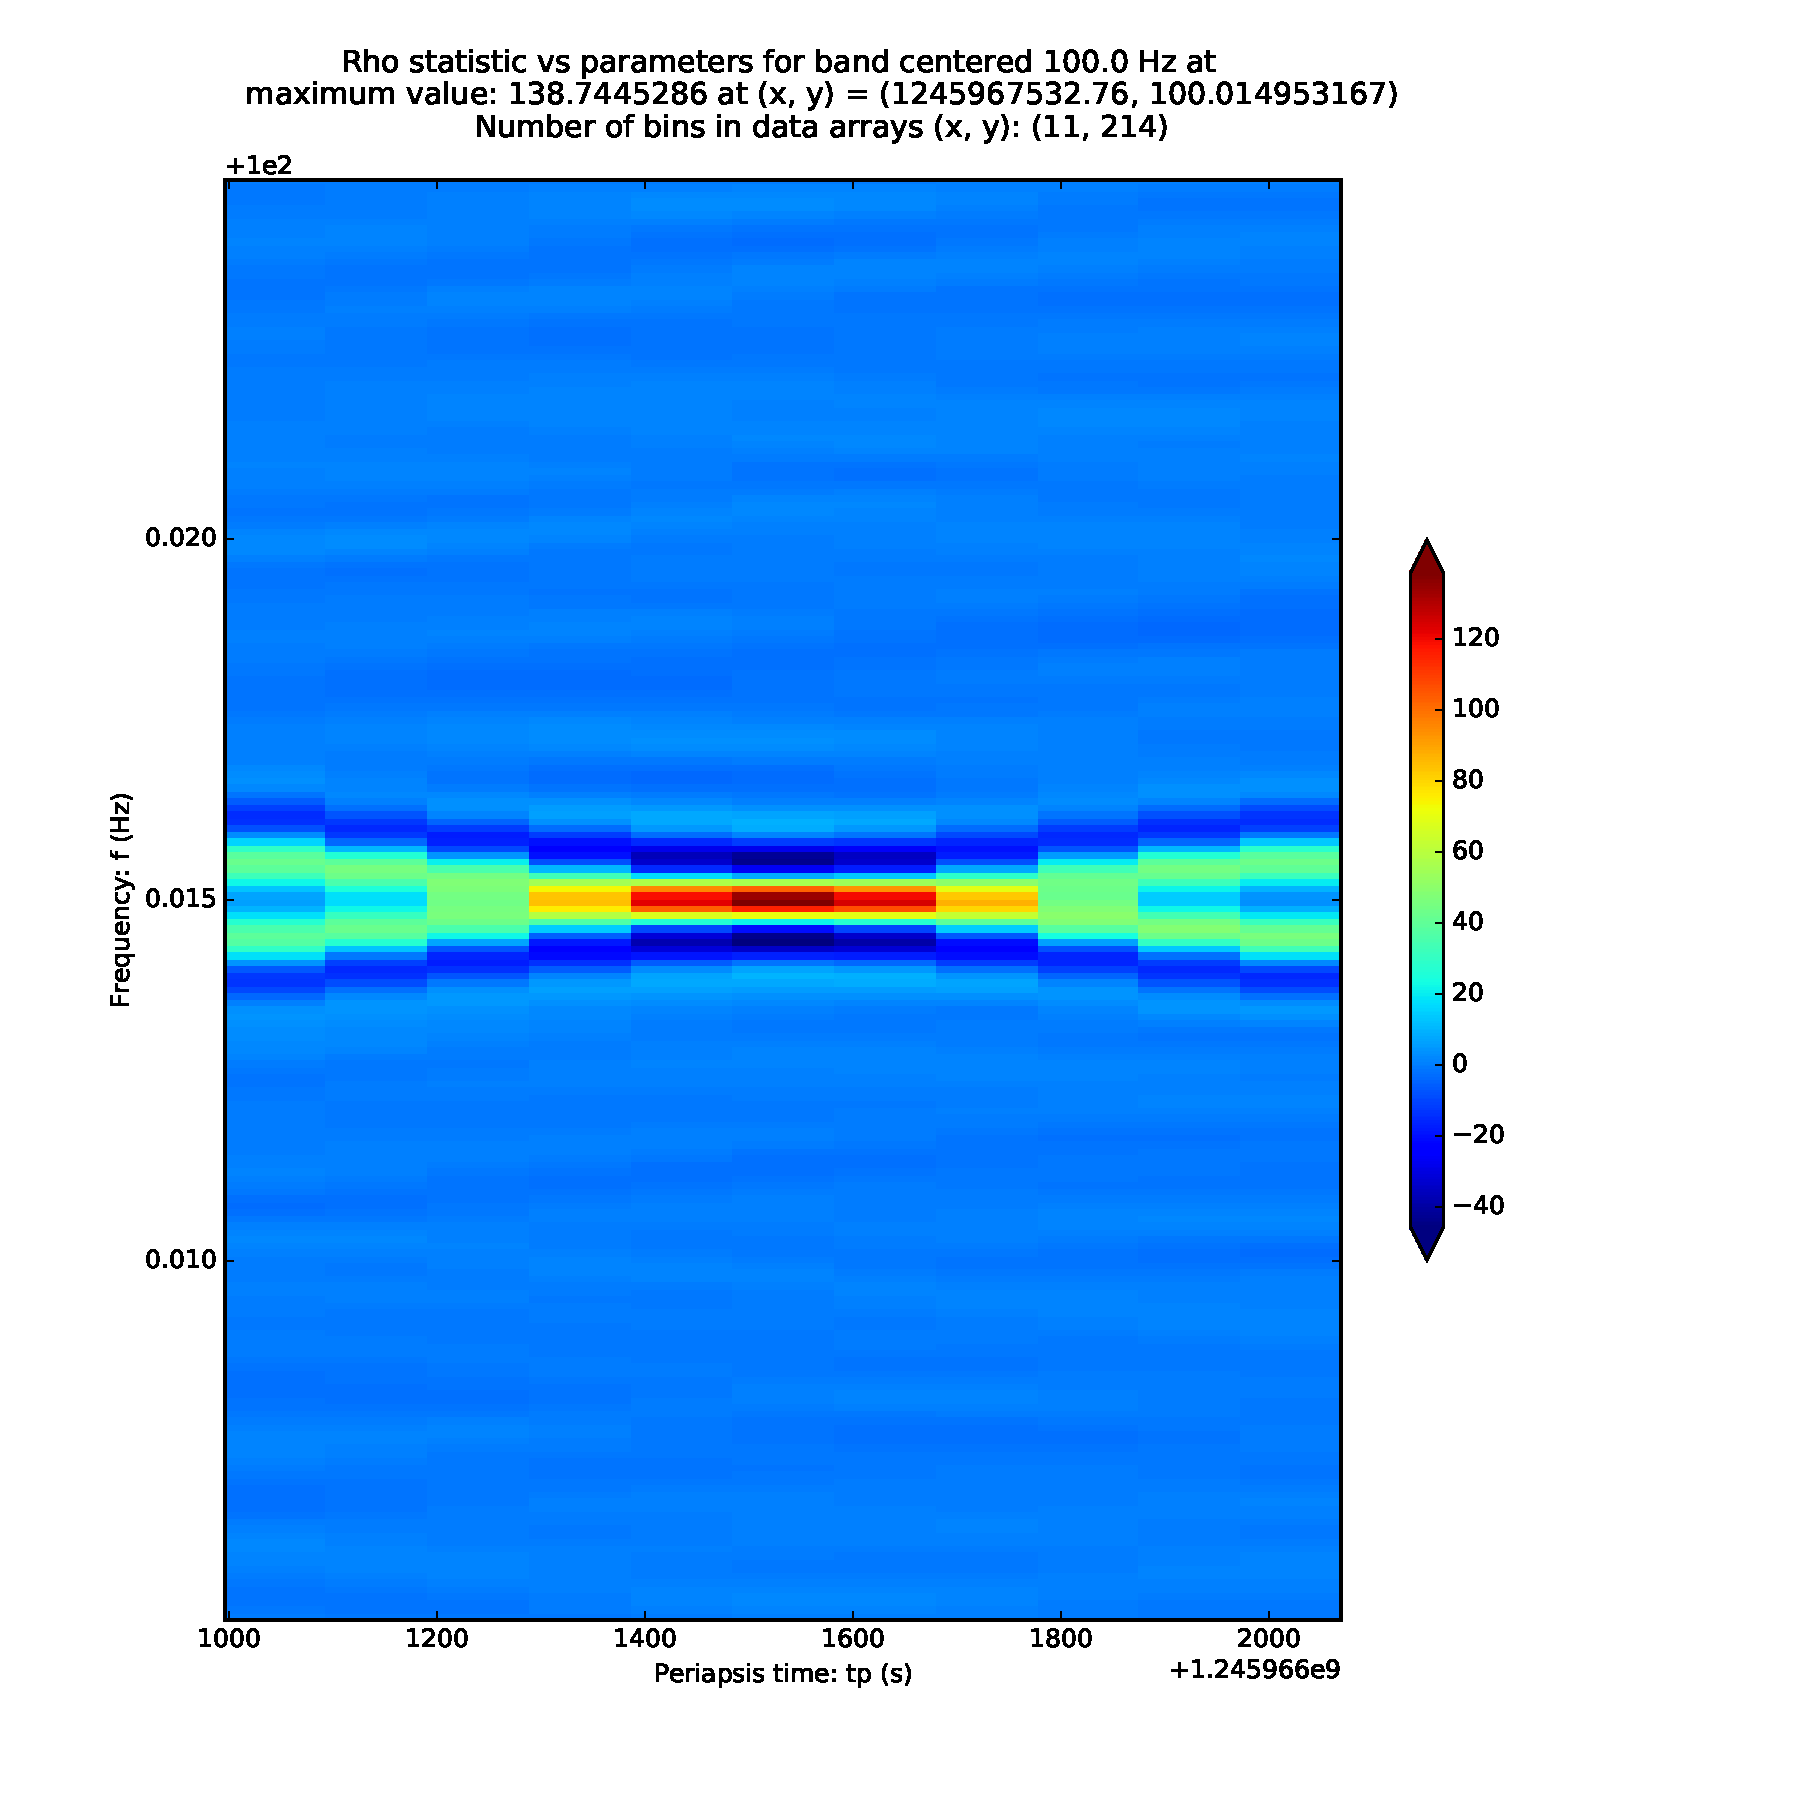
\includegraphics[trim= 0 0 0 0, clip, width=0.80\paperwidth,keepaspectratio]{plots/match-TS/TFresultsR-band-100-0.pdf}
\caption{
\url{<
https://www.atlas.aei.uni-hannover.de/~grant.meadors/LSC/ScoX1/2016/07/21-CrossCorr/match-TS/TFresultsR-band-100.0.pdf
>}
}
\label{TFcenterGraph}
\end{figure}

Figures~\ref{FAcenterGraph},~\ref{ATcenterGraph}, and~\ref{TFcenterGraph} respectively depict the $f$-$\Delta f_\mathrm{obs}$, $\Delta f_\mathrm{obs}$-$t_\mathrm{asc}$, and $t_\mathrm{asc}$-$f$ plane through the center of an injection. 
The FA plane shows an $X$-pattern, AT an ellitical peak, and TF another $X$ pattern with a different slope.
The maximum of each pattern is at the center of each graph (the injection site).

\subsection{Slices through offset planes}

Slices through 5-bin offsets are also shown (\textit{c.f.,} \texttt{note-on-offsets.txt}) in Figures~\ref{FAoffsetGraph},~\ref{AToffsetGraph},~\ref{TFoffsetGraph}, in the same order as before.
The 5-bin offset is equivalent to

\begin{itemize}
    \item $\delta f$ (frequency) = $4.7 \times 10^{-4}$ Hz,
    \item $\delta \Delta f_\mathrm{obs}$ (modulation depth) = $6.6 \times 10^{-4}$ Hz,
    \item $\delta t_\mathrm{asc}$ (time of ascension) = $537$ s.
\end{itemize}

\noindent The FA plane shows a hyperboloid with transverse axis parallel to the $f$-axis, the AT plane an open ring with maxima along an ellipse with transverse axis parallel to the $t_\mathrm{asc}$-axis, and the TF plane another hyperboloid with transverse axis parallel to the $f$-axis.

\begin{figure}
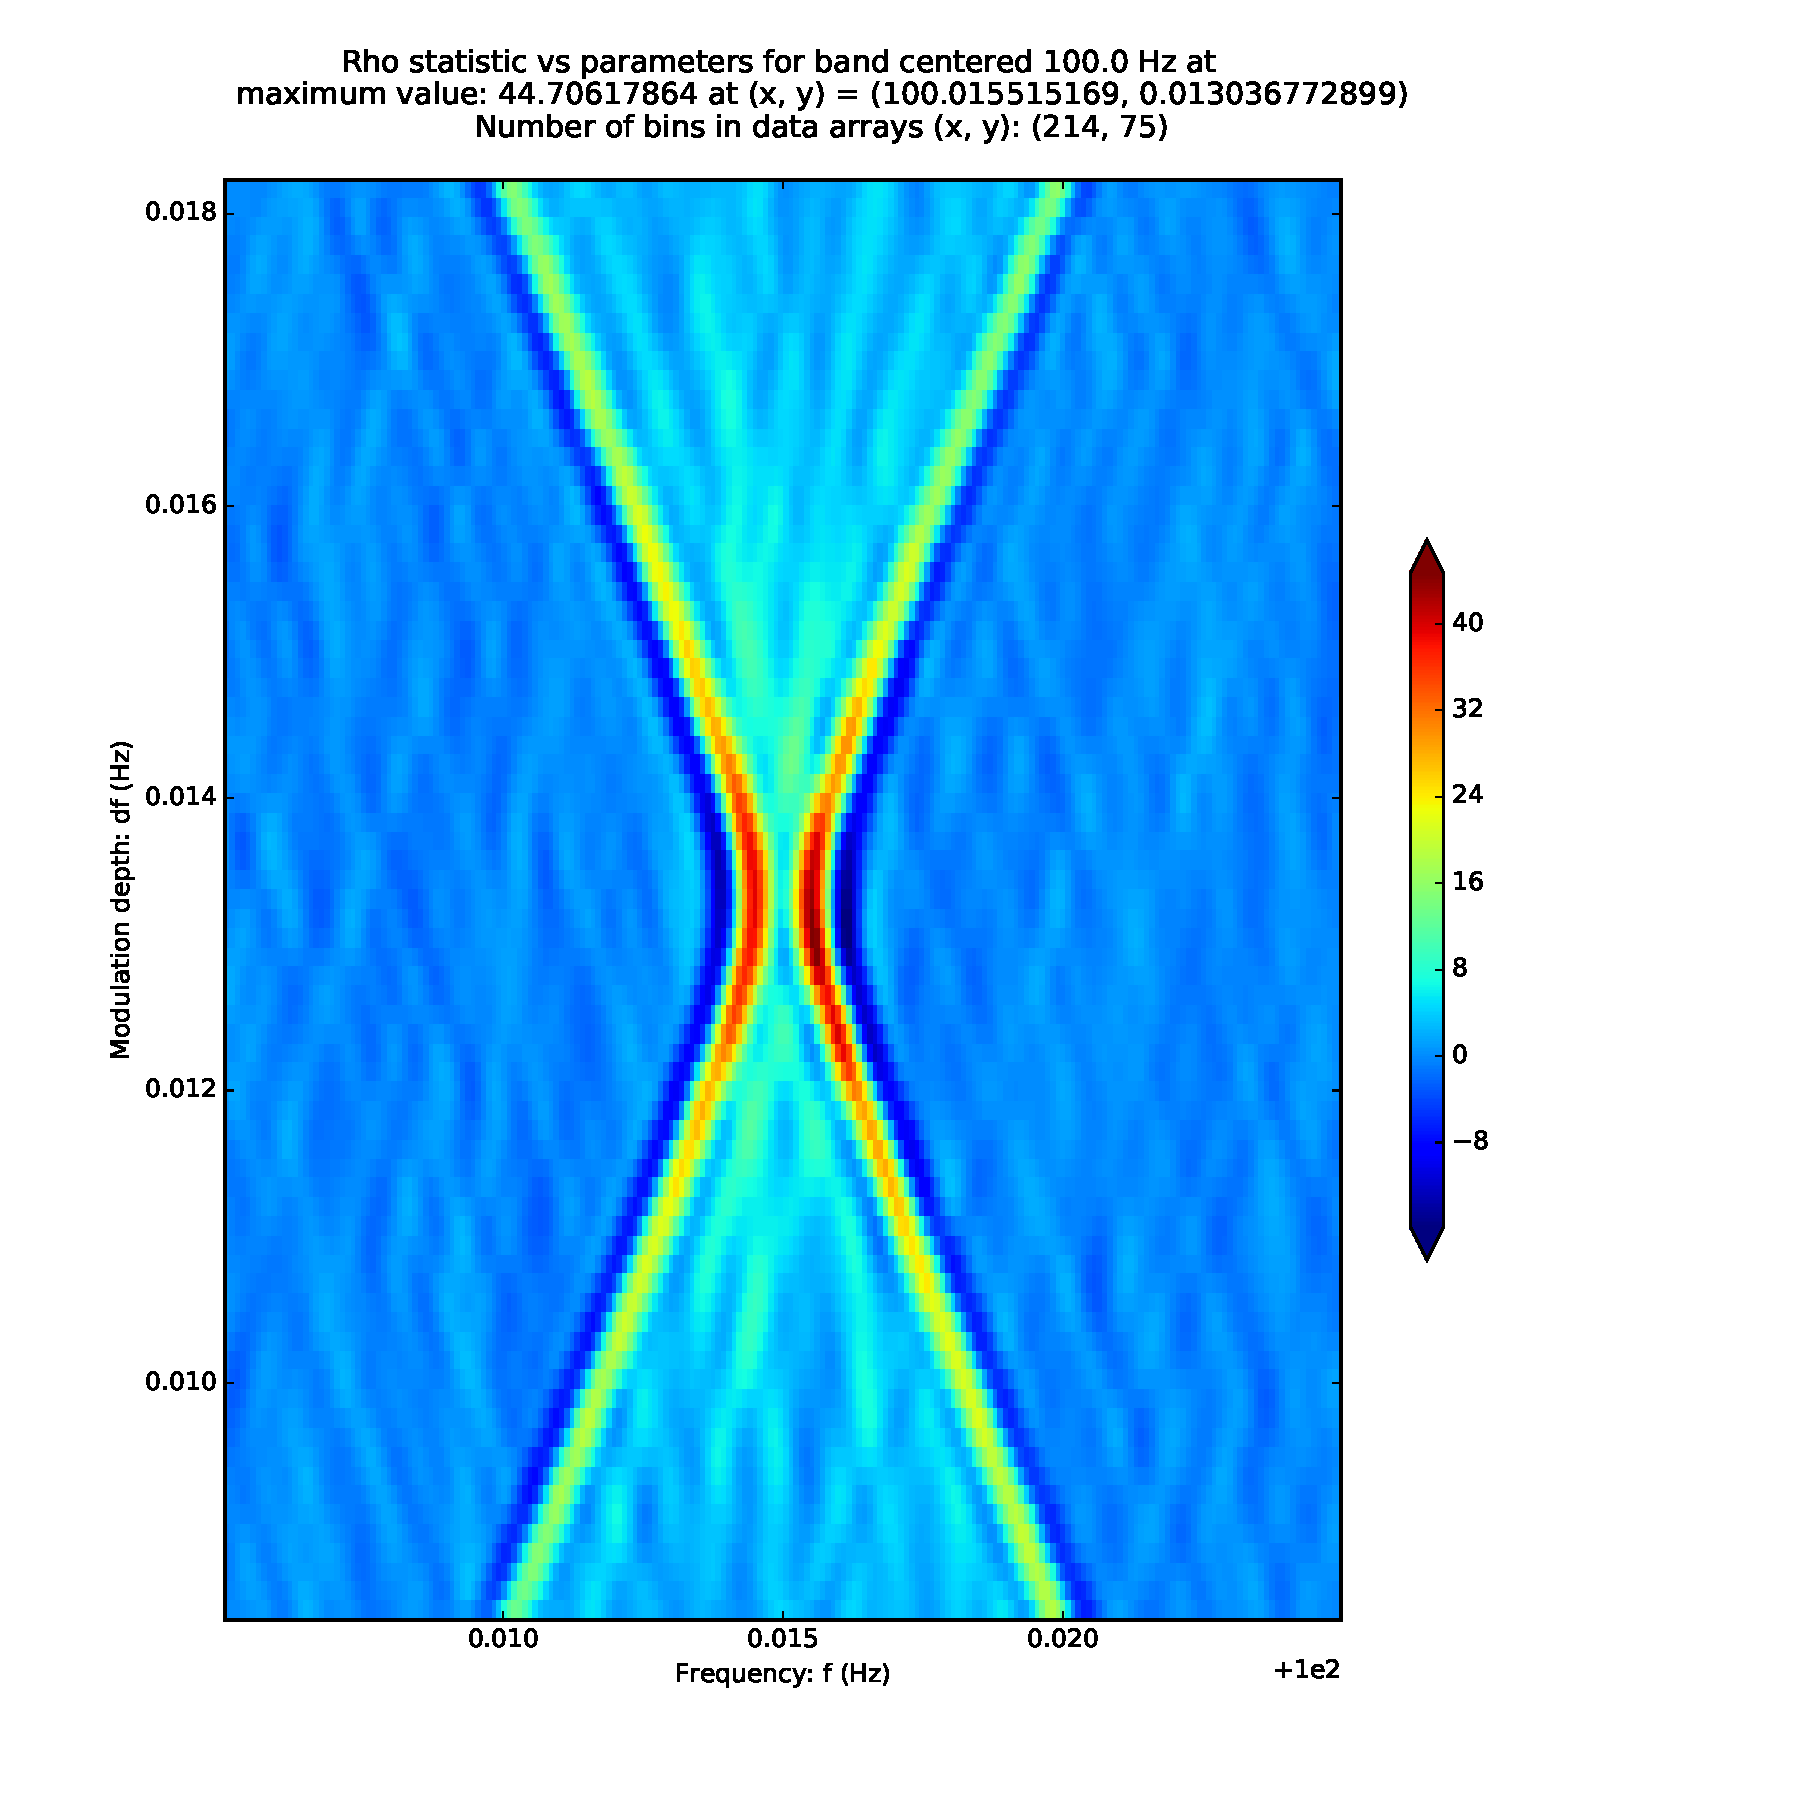
\includegraphics[trim= 0 0 0 0, clip, width=0.80\paperwidth,keepaspectratio]{plots/match-offset-TS/FAresultsR-band-100-0.pdf}
\caption{
\url{<
https://www.atlas.aei.uni-hannover.de/~grant.meadors/LSC/ScoX1/2016/07/21-CrossCorr/match-offset-TS/FAresultsR-band-100.0.pdf
>}
}
\label{FAoffsetGraph}
\end{figure}

\begin{figure}
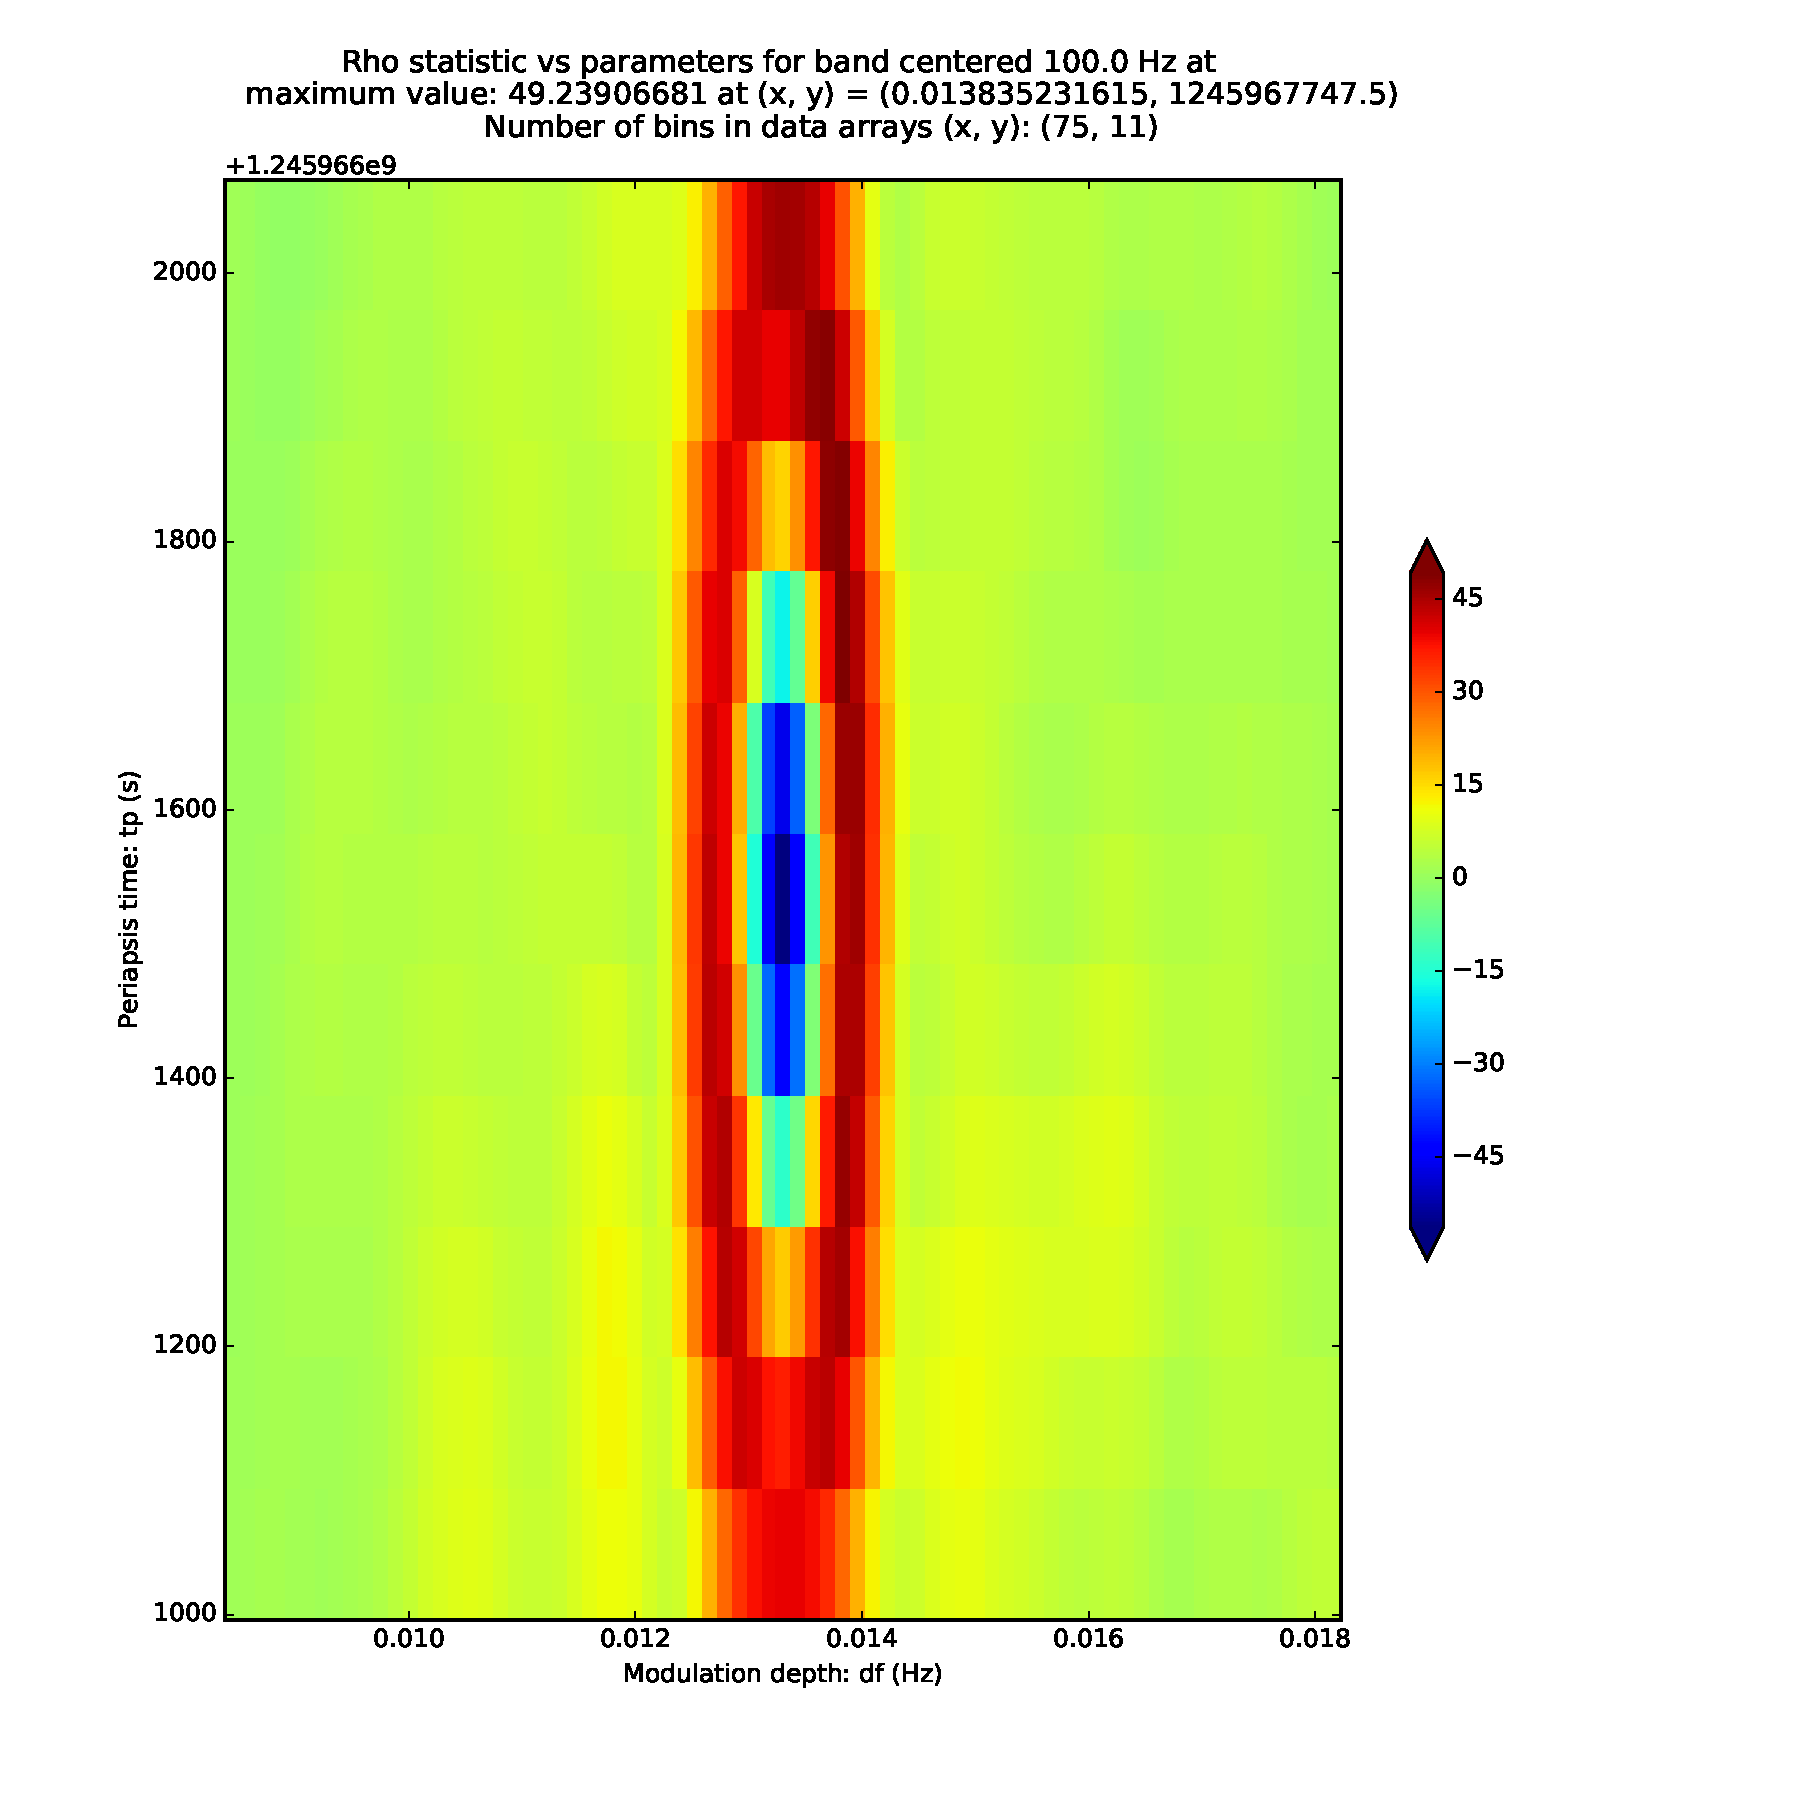
\includegraphics[trim= 0 0 0 0, clip, width=0.80\paperwidth,keepaspectratio]{plots/match-offset-TS/ATresultsR-band-100-0.pdf}
\caption{
\url{<
https://www.atlas.aei.uni-hannover.de/~grant.meadors/LSC/ScoX1/2016/07/21-CrossCorr/match-offset-TS/ATresultsR-band-100.0.pdf
>}
}
\label{AToffsetGraph}
\end{figure}

\begin{figure}
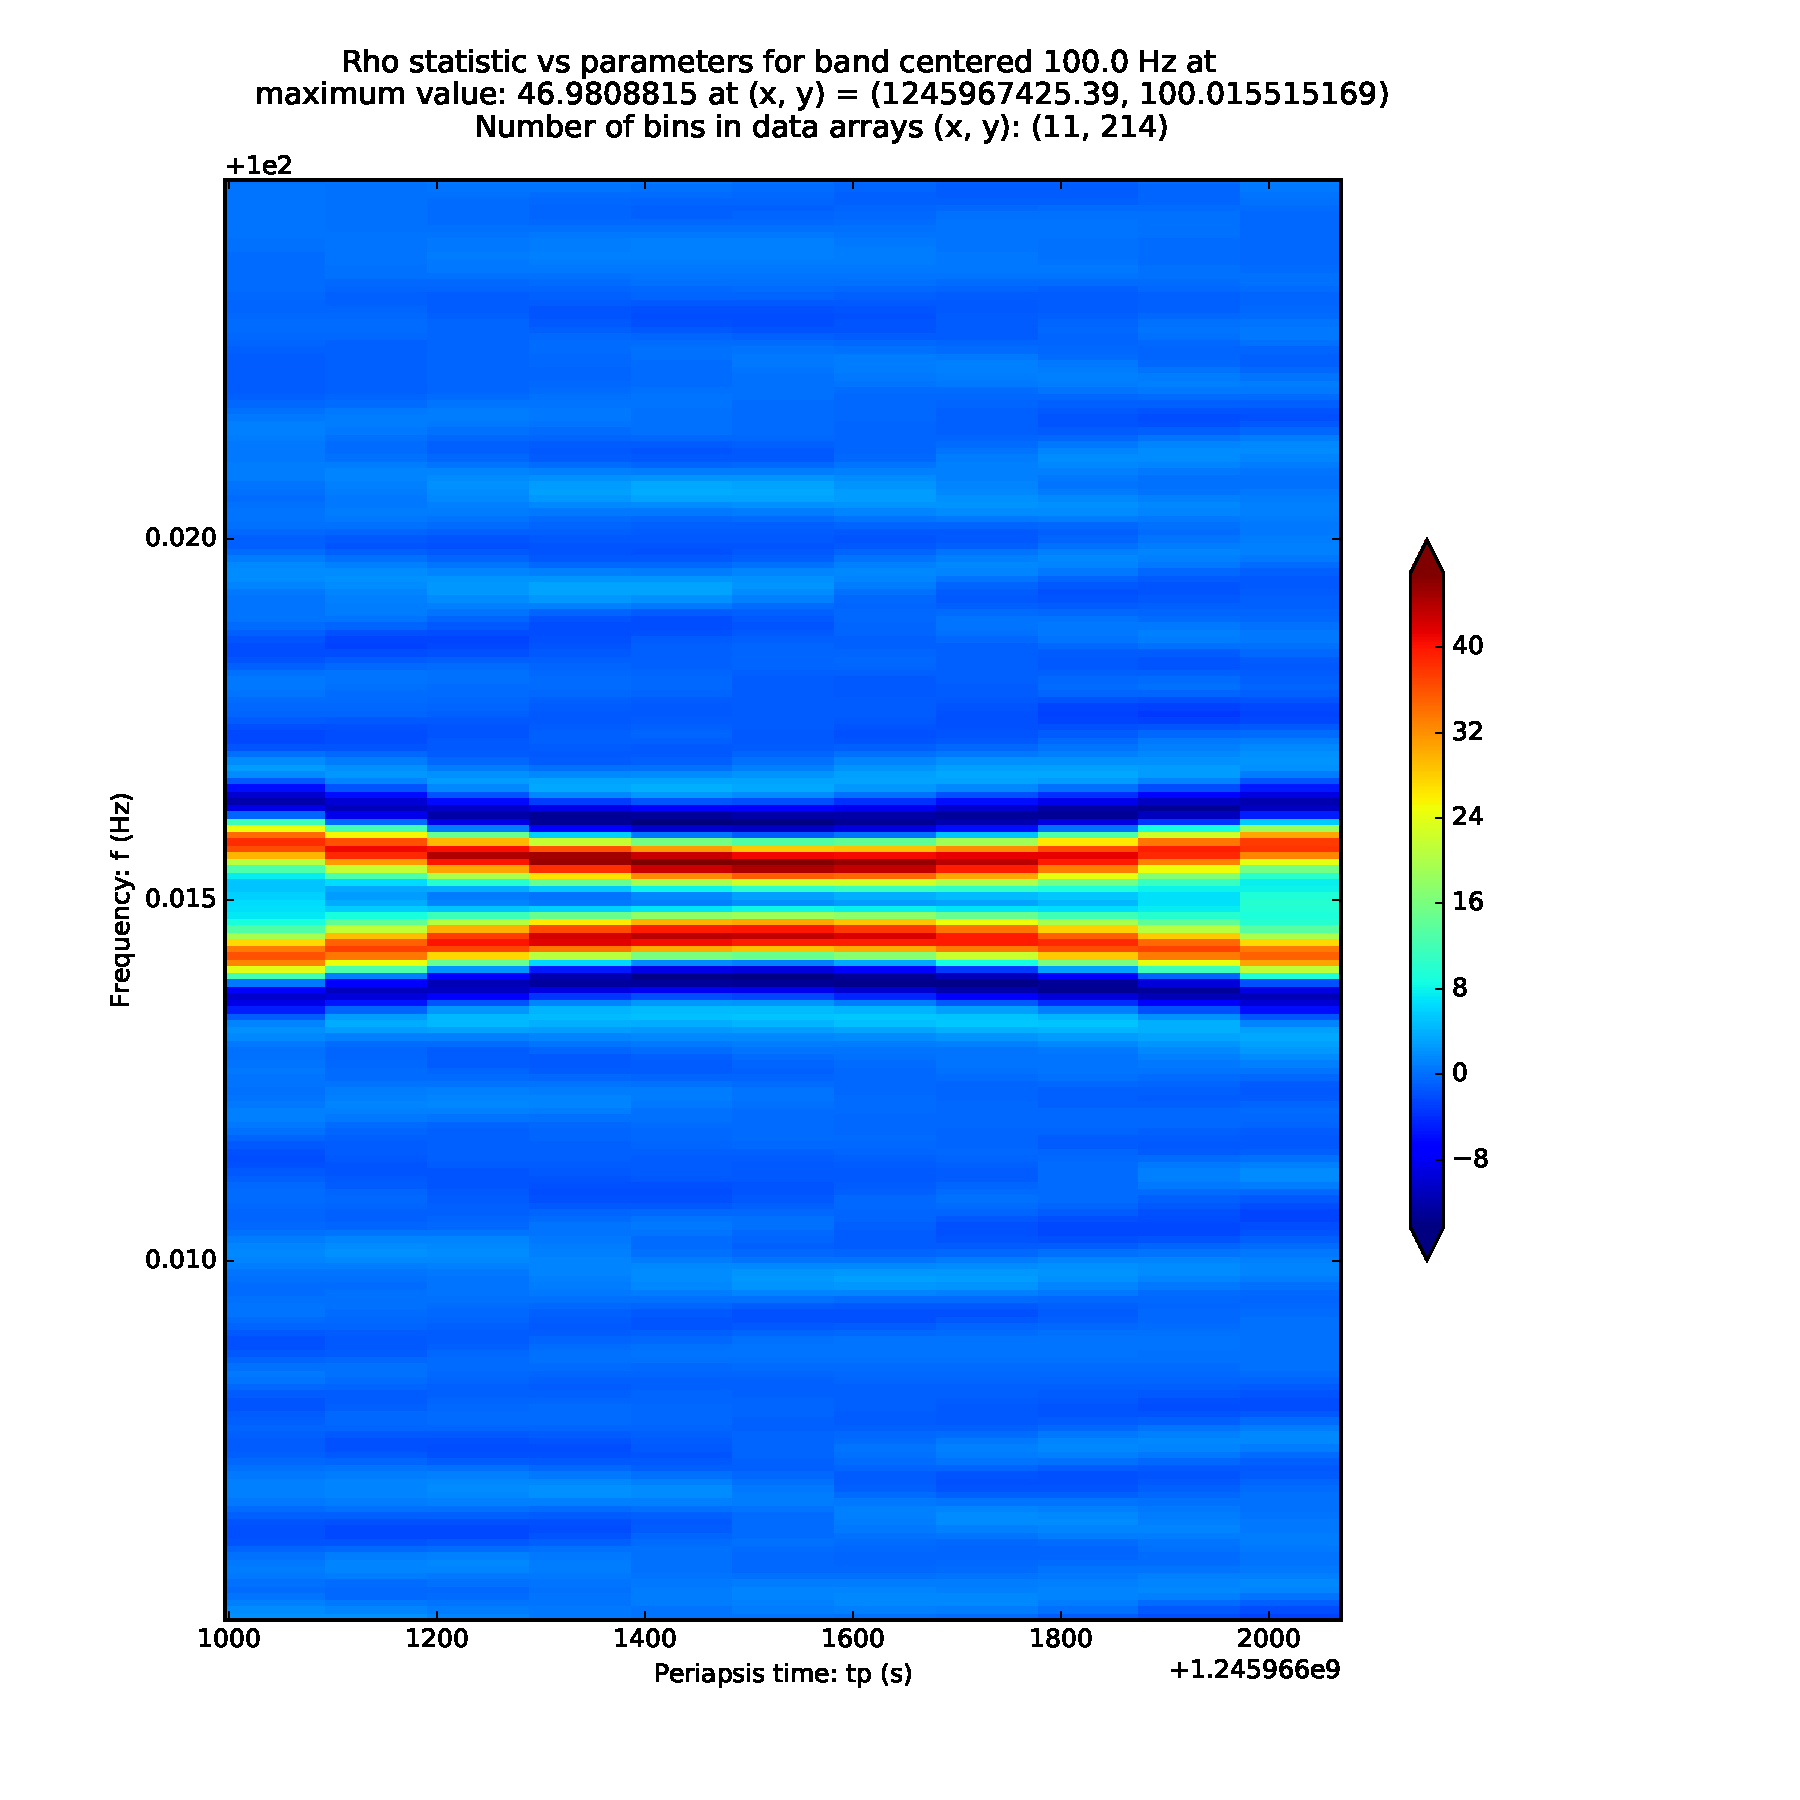
\includegraphics[trim= 0 0 0 0, clip, width=0.80\paperwidth,keepaspectratio]{plots/match-offset-TS/TFresultsR-band-100-0.pdf}
\caption{
\url{<
https://www.atlas.aei.uni-hannover.de/~grant.meadors/LSC/ScoX1/2016/07/21-CrossCorr/match-offset-TS/TFresultsR-band-100.0.pdf
>}
}
\label{TFoffsetGraph}
\end{figure}

\section{Interpretation}

The conic sections observed in Figures~\ref{FAcenterGraph} through~\ref{TFoffsetGraph} indicate that the three-dimensional surface of maximal $\rho$ is a double-cone, centered at the injection parameters.
Since the behavior of $\rho$ near the injection is well-described by the metric in the methods paper, let us focus on the extended cone.
When clarity is needed, true injection parameters are subscribed with zero (\textit{e.g.,} $f_0$).

\subsection{Heuristic approach}

Begin by considering the \textit{time-frequency} plane -- a spectogram, or plot of Short Fourier Transform bin powers over time -- of a solar-system barycentered signal.
Although power is concentrated in the extremal frequencies ($f_0 \pm \Delta f_\mathrm{obs}$) when averaged over time, as in the amplitude spectral density or an FFT over times of the \textit{time-frequency} plane, in the plane itself, the bins have comparitively uniform power.

Turning to the graphs: in the FA plane, the $X$-slope $d \Delta f_\mathrm{obs} / df = \pm1$.
This slope is identical to the $X$ in TwoSpect.
Its origin is described in depth in the TwoSpect directed methods paper.
When $f$ is offset by $\delta f$ and other parameters remain the same, the signal is lost.
However, if $\Delta f_\mathrm{obs}$ is also offset by $|\pm \delta \Delta f_\mathrm{obs}| = \delta f$, then the maximum (or minimum) frequency of the signal, $f_0 \pm \Delta f_\mathrm{obs}$, will be sensed by a template. 
Note also that when $\delta t_\mathrm{asc} \neq 0$, the true parameters miss the extrema; we deal with this more rigorously later.
In units of projected semi-major axis,

\begin{equation}
\frac{d (a \sin i)}{d f} = \frac{c P}{2 \pi f}.
\end{equation}

Observe next the TF plane.
By similar, phenomenological reasoning, we infer that the $X$-pattern is the result of contact between the rising (or falling) edges of the template with the true signal. 
Offset orbital phase $\delta t_\mathrm{asc}$ is compensated by shifting $\delta f$ so that the whole sinusoid moves parallel to the true signal.
The rising (or falling) edge of the \textit{time-frequency} sinusoid is caught when $\delta t_\mathrm{asc} = \pm \delta f / \max(df /dt)$.
When $\delta a_p \neq 0$, the true parameters miss the slope; we also deal with this more rigorously later.
Calculating $\pm \max \left(d f / d t\right)$ (identical results are obtained, up to a sign, by extremizing $t_\mathrm{asc}$),

\begin{eqnarray}
  \frac{df}{dt}
      &=& \frac{d}{dt} \left(f_0 + \frac{2 \pi f_0 a_p}{P} \sin \left[\Omega(t - t_\mathrm{asc})\right]\right),\\
      &=& \left(\frac{4 \pi^2 f_0 a_p}{P^2} \right) \cos[\Omega(t - t_\mathrm{asc})]). \\
  \max \left(\frac{df}{dt} \right)
      &=& \frac{4 \pi^2 f_0 a_p}{P^2},\\
      &\approx& 1.23 \times 10^{-6} \mathrm{~Hz~s}^{-1}, \nonumber\\
      &~& \mid {f_0 = 100.015\mathrm{~Hz}, a_p = 1.44\mathrm{~s}, P = 68023.82\mathrm{~s} },\\
      &\approx& 1\mathrm{~mHz} / (1000\mathrm{~s}).
\end{eqnarray}

\noindent Such a slope is observed in Figure~\ref{TFcenterGraph}.

Last, the ellipse in the AT plane emerges from moving the point of contact between the template and the signal.
For $\delta f = 0$, variations $\delta \Delta f_\mathrm{obs}$ and $\delta t_\mathrm{asc}$ will cause signal loss.
If $\delta f \neq 0$, then the signal is already lost.
We have already explained how $\delta \Delta f_\mathrm{obs} = \pm \delta f$ or $\delta t_\mathrm{asc} = \pm \delta f / \max (df/dt)$ restore contact, respectively at the extremal frequencies $f = f_0 \pm \Delta f_\mathrm{obs}$ or at the rising and falling edges, $f = f_0$.
We see in Figure~\ref{AToffsetGraph} that any point can be chosen on the ellipse with semi-major axes $(\delta \Delta f_\mathrm{obs}, \delta t_\mathrm{asc}) = (\delta f, \delta f/ \max (df /dt))$.

In sum, we describe the CrossCorr structure as a cone, give by the following parametric equations:

\begin{eqnarray}
s \in (-\infty, +\infty),~\theta \in [0, 2 pi);
\end{eqnarray}

\begin{eqnarray}
\delta f                        &=& s, \label{fEq}\\
\delta \Delta f_\mathrm{obs} &=& s \times 1 \times \cos(\theta), \label{aEq}\\
\delta t_\mathrm{asc}                  &=& s \times \left(\max\left(\frac{df}{dt} \right)\right)^{-1} * \sin(\theta) \label{tEq},
\end{eqnarray}

\noindent The middle equation could equivalently be written

\begin{equation}
\delta a_p= s \times \frac{P}{2 \pi f_0} \times \cos(\theta).
\end{equation}

Likewise, the equation last expands to

\begin{equation}
\delta t_\mathrm{asc}    = s \times \frac{P^2}{(4 \pi^2 f_0 a_p)} \times \sin(\theta).
\end{equation}

\subsection{Periodicity in time of ascension}


At the largest scale, $t_\mathrm{asc}$ is periodic: $\rho(t_\mathrm{asc}) = \rho(t_\mathrm{asc} \mathrm{~mod~} P)$.
While we neglect this periodicity in our current studies, we expect that the full TF plane would show that the surface follows

\begin{equation}
\delta f = \max \left(\frac{df}{dt} \right) \frac{P}{2 \pi} \sin \left(\frac{P}{2 \pi} \delta t_\mathrm{asc} \right),
\end{equation}

\noindent of which the $\theta = \pi/2$ cases of Equations~\ref{fEq} and~\ref{tEq} are an approximation near $\delta t_\mathrm{asc} =0$.

\subsection{Alternate derivation from small errors}

Our problem can be approached more rigorously by considering small errors: $\epsilon_f$, $\epsilon_{a_p}$, $\epsilon_{t_\mathrm{asc}}$.
Beginning from the signal model in the \textit{time-frequency} plane:

\begin{eqnarray}
f & \approx & f_0 + \epsilon_f \\
                   &+& \frac{2\pi f_0}{P} \left[
                     a_p \sin(\Omega(t-t_\mathrm{asc}))
                   - \epsilon_{a_p} \sin(\Omega (t-t_\mathrm{asc}))
                   - a_p \Omega \epsilon_{t_\mathrm{asc}} \right]  \\
                   &+& \frac{2 \pi \epsilon_f}{P}  a_p  \sin(\Omega ( t-t_\mathrm{asc}))
\end{eqnarray}
\begin{eqnarray}
\max(f) &\approx& f_0 + \epsilon_f \\
                   &+&\frac{2 \pi f_0}{P}*\left[
                     a_p
                   - \epsilon_{a_p}
                   - \frac{2 \pi  a_p}{P} \epsilon_{t_\mathrm{asc}}\right] \\
                   &+& \mathcal{O}(0)
\end{eqnarray}

Where we see that the ratios of coefficients are the same as above. Call
equal $\Delta f$ errors $eq_f, eq_a, eq_t$:

\begin{eqnarray}
eq_a / eq_f &=& P / (2 pi f0)\\
eq_t / eq_f &=& P^2/(4 pi^2 f0 (a sin i))
\end{eqnarray}

which are the same coefficients as obtained for $(Asini' - a sin i)$ and
$(Tasc' - Tasc)$ above, where we reasoned from the 1st Fourier domain.

Long story short: the structures make sense.

You're welcome to include any of this material on a wiki, though I do
not know where on the wiki to put it. Also, please let me know if this
is old news (and already covered in the iPython notebooks).

%My scripts are
%    \texttt{wrapCrossCorr.py}
%      (wrapper function, itself called as in example-TwoSpect-like.txt)
%    \texttt{libCallCC.py}
%      (functions for the wrapper)
%    \texttt{createHeatmap.py}
%      (grapher)

NOTE: ADD material on why there are double-dots at $\pm$ some frequency around the central injection. My guess is that they are at one modulation depth away, and result from being in anti-phase somehow -- but it does not totally make sense. Investigate.

\newpage

\appendix
\section{Source code}
\label{source_code_appendix}

\subsection{example-TwoSpect-like.txt}
\lstinputlisting{scripts/example-TwoSpect-like.txt}
\subsection{wrapCrossCorr.py}
\lstinputlisting[language=Python]{scripts/wrapCrossCorr.py}
\subsection{libCallCC.py}
\lstinputlisting[language=Python]{scripts/libCallCC.py}
\subsection{createHeatmap.py}
\lstinputlisting[language=Python]{scripts/createHeatmap.py}


\end{document}
